\documentclass[a4paper,11pt]{article}

% --- PREAMBOLO ---
\usepackage[utf8]{inputenc}
\usepackage[italian]{babel}
\usepackage[T1]{fontenc}
\usepackage[margin=1.2cm, bottom=2cm]{geometry}
\usepackage{subcaption} 
\usepackage[colorlinks=true, linkcolor=black]{hyperref}
\usepackage{float}
\usepackage{parskip}
\usepackage{tabularx}
\usepackage{booktabs}
\usepackage{enumitem}
\usepackage{array}
\usepackage{graphicx}
\usepackage{xcolor}      
\usepackage{tabularray}  
\usepackage[italian]{cleveref} % Per riferimenti automatici eleganti

% Percorso delle immagini
\graphicspath{{img/}}

% Configurazione didascalie
\captionsetup[figure]{font=small, labelfont=bf, position=top, margin=1cm}

% --- DATI DEL DOCUMENTO ---
\title{Ingegneria del Software\\ \Large SunSpot: Gestionale per la prenotazione digitale di stabilimenti balneari} 
\author{Leonardo Soldani - 7139732}
\date{Marzo 2026} 

% --- INIZIO DOCUMENTO ---
\begin{document}

\maketitle

\renewcommand{\contentsname}{Indice}
\tableofcontents
\newpage

\pagestyle{plain}
\setcounter{page}{1}

\section{Introduzione}
Il progetto SunSpot nasce dall'esigenza di digitalizzare e modernizzare il settore degli stabilimenti balneari, un ambito che ancora oggi mostra una certa resistenza all'adozione di piattaforme web integrate. L'obiettivo principale è fornire un'infrastruttura capace di permettere all'utente di prenotare in modo rapido e intuitivo un ombrellone presso uno dei lidi aderenti al servizio, trasformando la pianificazione di una giornata al mare in un'operazione a portata di click.

Il sistema è stato progettato con l'idea di soddisfare le esigenze di tre tipologie di utenti: 
\begin{itemize}
	\item \textbf{Utente finale (Customer)}: a cui viene fornita la possibilità di prenotare uno o più ombrelloni o tende con la possibilità di personalizzare la propria esperienza richiedendo lettini, sedie, sdraio extra e cabine.
	\item \textbf{Gestore stabilimento (Owner)}: che dispone di innumerevoli funzionalità per la personalizzazione della propria spiaggia virtuale, partendo da una sezione per poter pubblicizzare i propri servizi arrivando alla possibilità di suddividere il proprio stabilimento in diverse aree di prezzo.
	\item \textbf{Admin (Gestore dell'applicazione)}: con lo scopo di regolare e controllare l'ambiente commerciale messo a disposizione di gestori e utenti finali. Si occupa dell'inserimento della spiaggia all'interno dell'ambiente e del rispettivo gestore, oltre ad applicare sanzioni (ban) qualora ce ne fosse necessità.
\end{itemize}

Per garantire un ecosistema sicuro e affidabile, SunSpot integra un sistema di regolazione basato su recensioni verificate e un meccanismo di segnalazione (report) tra utenti e gestori, volto a preservare l'integrità del servizio e a migliorare costantemente l'esperienza d'uso per tutti gli attori coinvolti.

\section{Ambiente e tecnologie utilizzate}
L'applicazione è stata sviluppata utilizzando le seguenti tecnologie:

\subsection{Linguaggio e Tool di Build}
\begin{itemize}
    \item \textbf{Java 25} - Scelto per l'utilizzo delle funzionalità più recenti della JDK.
    \item \textbf{Maven 3.8.5} - Strumento di build e gestione delle dipendenze.
\end{itemize}

\subsection{Database e Persistenza}
\begin{itemize}
    \item \textbf{MySQL 8.3.0} - Database relazionale utilizzato per la persistenza dei dati.
    \item \textbf{MySQL Connector/J} - Driver ufficiale per la gestione della connessione al database.
\end{itemize}

\subsection{Librerie e Containerizzazione}
\begin{itemize}
    \item \textbf{BCrypt 0.10.2} - Utilizzata per l'hashing e la gestione sicura delle password.
    \item \textbf{Docker \& Docker Compose 3.8} - Utilizzati per containerizzare il database MySQL, garantendo un ambiente di esecuzione isolato, persistente e facilmente riproducibile.
\end{itemize}

\subsection{Testing e Analisi}
\begin{itemize}
    \item \textbf{JUnit 5.12.1} - Framework per l'esecuzione dei test unitari.
    \item \textbf{Mockito 5.23.0} - Utilizzato per la simulazione di dipendenze durante i test (mocking).
    \item \textbf{JUnit Platform Suite} - Strumento per l'organizzazione e l'esecuzione dei test.
\end{itemize}

\section{Use Case}
I seguenti template descrivono alcuni dei principali casi d’uso identificati per l’applicazione durante la fase di analisi e progettazione. Ogni caso d’uso è descritto utilizzando una struttura standardizzata: ID, Nome, Attori, Descrizione, Precondizioni, Postcondizioni, Flusso principale, Flussi alternativi e Business Rules.

\newpage

\section{Database}
Per la gestione della persistenza dei dati è stato utilizzato il DBMS \textbf{MySQL}, configurato all'interno di un ambiente di containerizzazione \textbf{Docker}. L'interazione tra l'applicazione Java e il database avviene tramite l'interfaccia \textbf{JDBC}, utilizzando il driver ufficiale \textbf{MySQL Connector/J}.

L'integrità del dato è assicurata a livello nativo attraverso una rigorosa definizione di vincoli (Foreign Key, Unique e Check) implementati nello script di creazione. Tale approccio permette di delegare al database la validazione delle informazioni critiche, mentre le verifiche legate alla \textbf{logica di business} sono gestite programmaticamente all'interno del codice Java dell'applicazione.

\subsection{Modello ER}
Il modello Entity-Relationship (\cref{fig:modelloER}) omette la relazione diretta tra \textit{Beaches} e \textit{Bookings} per evitare ridondanze concettuali, essendo il legame già mediato dalle entità \textit{Zones} e \textit{Spots}. In fase di implementazione del database fisico, tuttavia, tale relazione è stata introdotta per ottimizzare le performance delle query di ricerca, riducendo la complessità delle operazioni di join.

\begin{figure}[H] 
    \centering
    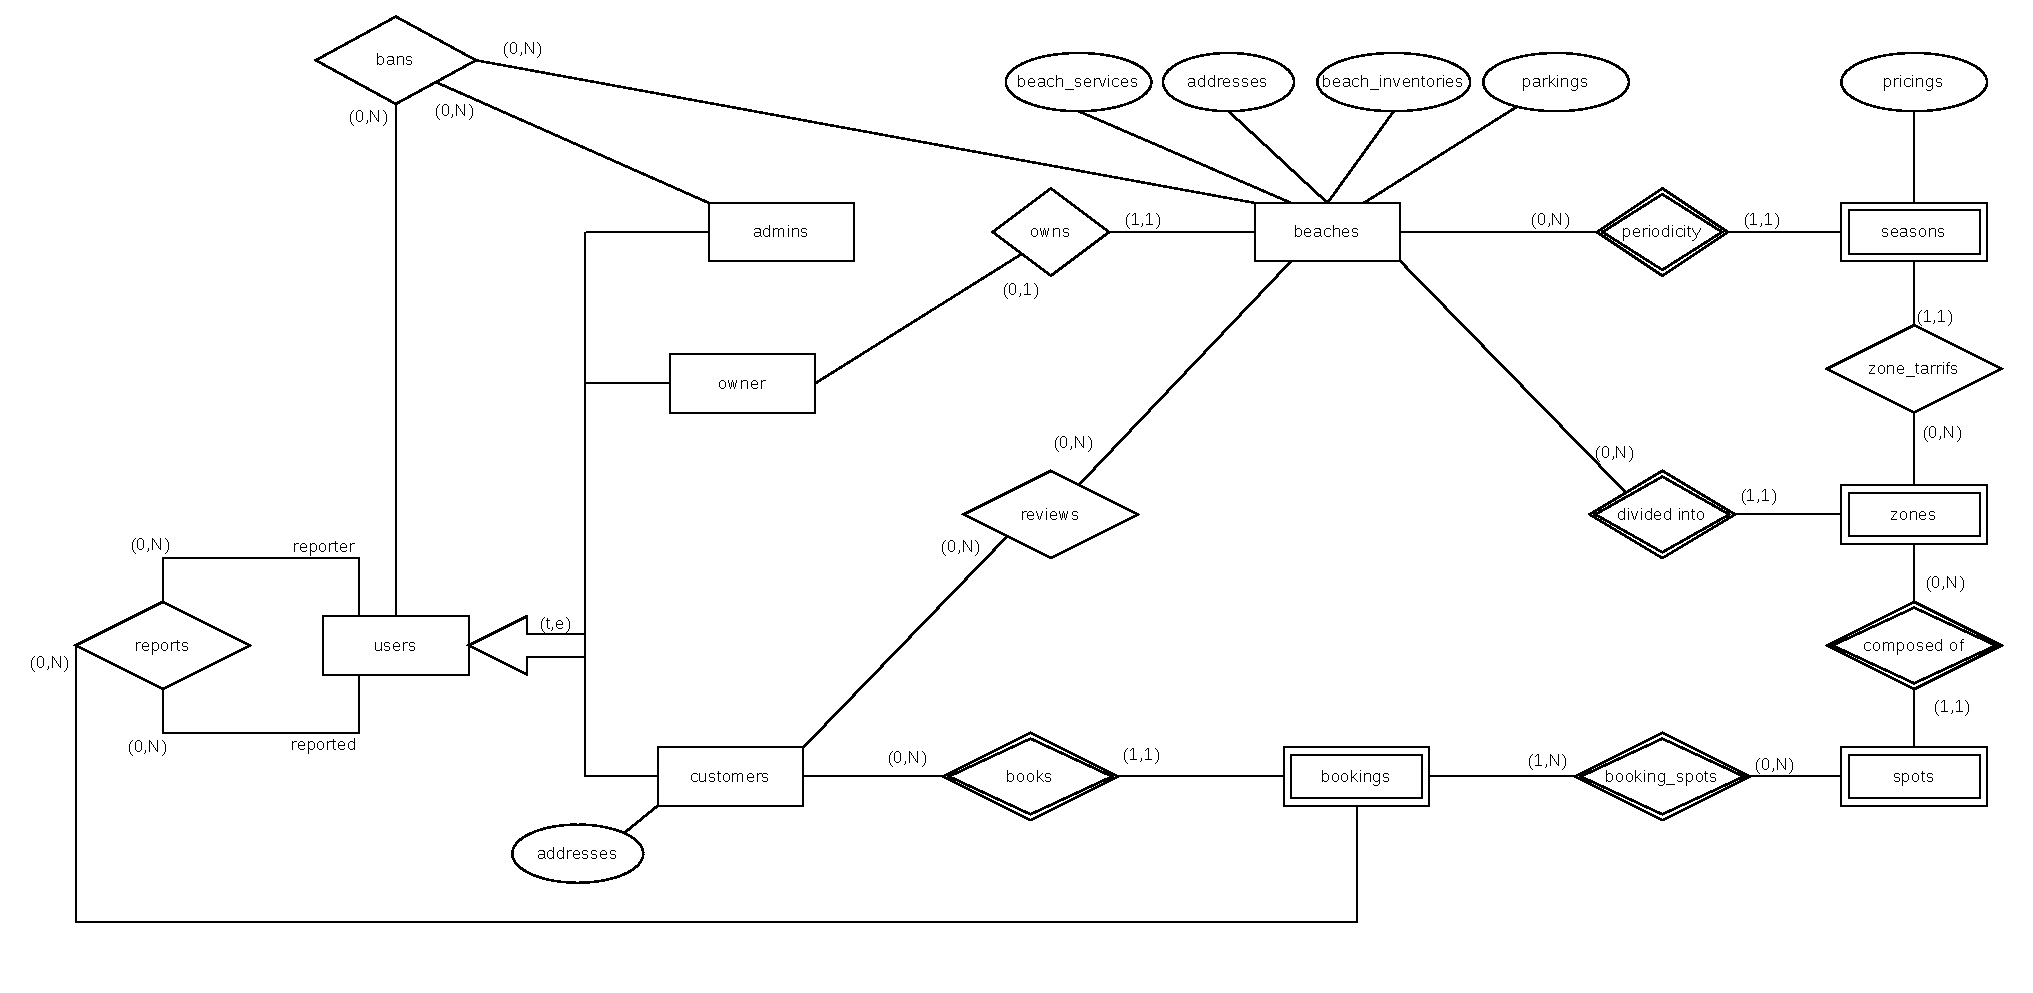
\includegraphics[width=1.0\textwidth]{ModelloER.pdf} 
    \caption{Modello Entity Relationship (Schema Concettuale)}
    \label{fig:modelloER}
\end{figure}

\vspace{0.5cm}

\subsection{Dizionario dei dati}
Il dizionario (\cref{fig:diz_entita,fig:diz_relazioni}) presenta per \textit{Spots} e \textit{Bookings} attributi identificativi esterni derivanti dalle relazioni con altre entità, che dovrebbero svolgere il ruolo di chiave primaria per le entità citate. Per semplificare le interrogazioni e la realizzazione del db si è optato per l'utilizzo di una chiave primaria artificiale (\textit{id}), preservando la valenza identificativa di questi attributi tramite vincoli \texttt{UNIQUE} e \texttt{NOT NULL}, come dettagliato nella tabella dei vincoli (\cref{fig:tab_vincoli}).

\begin{figure}[H]
    \centering
    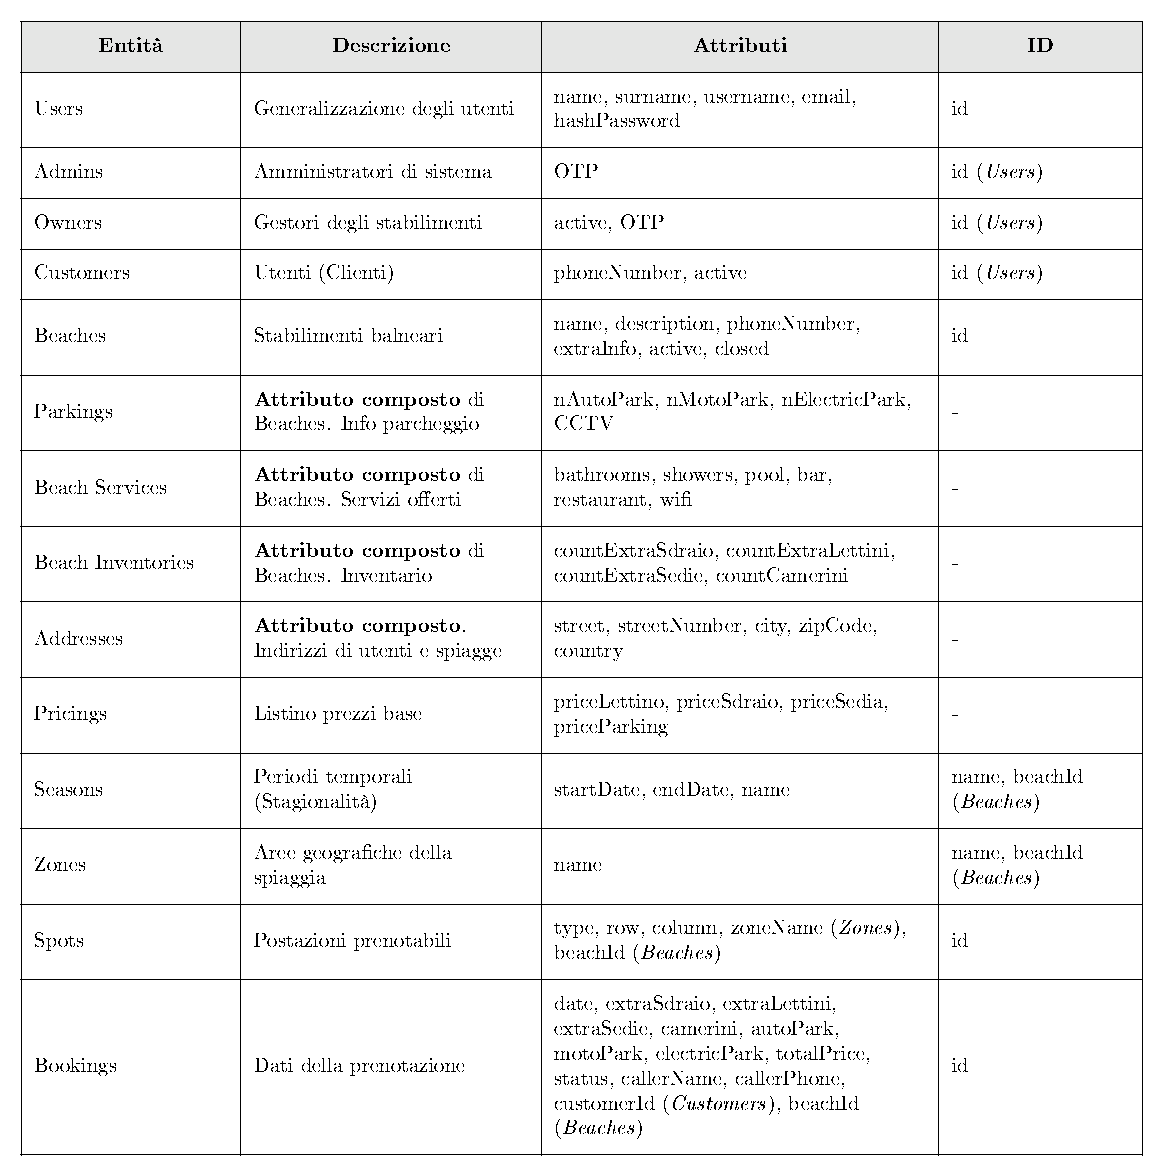
\includegraphics[width=0.9\textwidth]{DataBase/Dizionario/Entità}
    \caption{Dizionario delle Entità}
    \label{fig:diz_entita}
\end{figure}

\vspace{0.5cm}

\begin{figure}[H]
    \centering
    \includegraphics[width=0.9\textwidth]{DataBase/Dizionario/relazioni}
    \caption{Dizionario delle Relazioni}
    \label{fig:diz_relazioni}
\end{figure}

\vspace{0.5cm}

\subsection{Tabelle delle Regole}
Di seguito vengono riportati i vincoli di integrità e le regole di derivazione che governano la logica della persistenza dei dati.
In merito alla regola di RD1 (\cref{fig:tab_derivazioni}), si è scelta la persistenza dell'attributo \textit{totalPrice} nel database, al fine di ridurre il carico computazionale di consultazione dei dati.

\begin{figure}[H] 
    \centering
    \includegraphics[width=0.9\textwidth]{DataBase/Tabelle/vincoli}
    \caption{Tabella dei vincoli di integrità (RV)}
    \label{fig:tab_vincoli}
\end{figure}

\vspace{0.5cm}

\begin{figure}[H] 
    \centering
    \includegraphics[width=0.9\textwidth]{DataBase/Tabelle/derivazioni} 
    \caption{Tabella delle regole di derivazione (RD)}
    \label{fig:tab_derivazioni}
\end{figure}


\end{document}